\documentclass[twoside]{book}

% Packages required by doxygen
\usepackage{fixltx2e}
\usepackage{calc}
\usepackage{doxygen}
\usepackage[export]{adjustbox} % also loads graphicx
\usepackage{graphicx}
\usepackage[utf8]{inputenc}
\usepackage{makeidx}
\usepackage{multicol}
\usepackage{multirow}
\PassOptionsToPackage{warn}{textcomp}
\usepackage{textcomp}
\usepackage[nointegrals]{wasysym}
\usepackage[table]{xcolor}

% Font selection
\usepackage[T1]{fontenc}
\usepackage[scaled=.90]{helvet}
\usepackage{courier}
\usepackage{amssymb}
\usepackage{sectsty}
\renewcommand{\familydefault}{\sfdefault}
\allsectionsfont{%
  \fontseries{bc}\selectfont%
  \color{darkgray}%
}
\renewcommand{\DoxyLabelFont}{%
  \fontseries{bc}\selectfont%
  \color{darkgray}%
}
\newcommand{\+}{\discretionary{\mbox{\scriptsize$\hookleftarrow$}}{}{}}

% Page & text layout
\usepackage{geometry}
\geometry{%
  a4paper,%
  top=2.5cm,%
  bottom=2.5cm,%
  left=2.5cm,%
  right=2.5cm%
}
\tolerance=750
\hfuzz=15pt
\hbadness=750
\setlength{\emergencystretch}{15pt}
\setlength{\parindent}{0cm}
\setlength{\parskip}{3ex plus 2ex minus 2ex}
\makeatletter
\renewcommand{\paragraph}{%
  \@startsection{paragraph}{4}{0ex}{-1.0ex}{1.0ex}{%
    \normalfont\normalsize\bfseries\SS@parafont%
  }%
}
\renewcommand{\subparagraph}{%
  \@startsection{subparagraph}{5}{0ex}{-1.0ex}{1.0ex}{%
    \normalfont\normalsize\bfseries\SS@subparafont%
  }%
}
\makeatother

% Headers & footers
\usepackage{fancyhdr}
\pagestyle{fancyplain}
\fancyhead[LE]{\fancyplain{}{\bfseries\thepage}}
\fancyhead[CE]{\fancyplain{}{}}
\fancyhead[RE]{\fancyplain{}{\bfseries\leftmark}}
\fancyhead[LO]{\fancyplain{}{\bfseries\rightmark}}
\fancyhead[CO]{\fancyplain{}{}}
\fancyhead[RO]{\fancyplain{}{\bfseries\thepage}}
\fancyfoot[LE]{\fancyplain{}{}}
\fancyfoot[CE]{\fancyplain{}{}}
\fancyfoot[RE]{\fancyplain{}{\bfseries\scriptsize Generated by Doxygen }}
\fancyfoot[LO]{\fancyplain{}{\bfseries\scriptsize Generated by Doxygen }}
\fancyfoot[CO]{\fancyplain{}{}}
\fancyfoot[RO]{\fancyplain{}{}}
\renewcommand{\footrulewidth}{0.4pt}
\renewcommand{\chaptermark}[1]{%
  \markboth{#1}{}%
}
\renewcommand{\sectionmark}[1]{%
  \markright{\thesection\ #1}%
}

% Indices & bibliography
\usepackage{natbib}
\usepackage[titles]{tocloft}
\setcounter{tocdepth}{3}
\setcounter{secnumdepth}{5}
\makeindex

% Hyperlinks (required, but should be loaded last)
\usepackage{ifpdf}
\ifpdf
  \usepackage[pdftex,pagebackref=true]{hyperref}
\else
  \usepackage[ps2pdf,pagebackref=true]{hyperref}
\fi
\hypersetup{%
  colorlinks=true,%
  linkcolor=blue,%
  citecolor=blue,%
  unicode%
}

% Custom commands
\newcommand{\clearemptydoublepage}{%
  \newpage{\pagestyle{empty}\cleardoublepage}%
}

\usepackage{caption}
\captionsetup{labelsep=space,justification=centering,font={bf},singlelinecheck=off,skip=4pt,position=top}

%===== C O N T E N T S =====

\begin{document}

% Titlepage & ToC
\hypersetup{pageanchor=false,
             bookmarksnumbered=true,
             pdfencoding=unicode
            }
\pagenumbering{alph}
\begin{titlepage}
\vspace*{7cm}
\begin{center}%
{\Large Z\+OO Game }\\
\vspace*{1cm}
{\large Generated by Doxygen 1.8.13}\\
\end{center}
\end{titlepage}
\clearemptydoublepage
\pagenumbering{roman}
\tableofcontents
\clearemptydoublepage
\pagenumbering{arabic}
\hypersetup{pageanchor=true}

%--- Begin generated contents ---
\chapter{Hierarchical Index}
\section{Class Hierarchy}
This inheritance list is sorted roughly, but not completely, alphabetically\+:\begin{DoxyCompactList}
\item \contentsline{section}{Hra}{\pageref{class_hra}}{}
\item \contentsline{section}{Inventar}{\pageref{class_inventar}}{}
\item \contentsline{section}{Lod}{\pageref{class_lod}}{}
\item \contentsline{section}{Mapa}{\pageref{class_mapa}}{}
\item \contentsline{section}{Obrana}{\pageref{class_obrana}}{}
\begin{DoxyCompactList}
\item \contentsline{section}{Silna\+Obrana}{\pageref{class_silna_obrana}}{}
\item \contentsline{section}{Slaba\+Obrana}{\pageref{class_slaba_obrana}}{}
\end{DoxyCompactList}
\item \contentsline{section}{Pirat}{\pageref{class_pirat}}{}
\item \contentsline{section}{Planeta}{\pageref{class_planeta}}{}
\item \contentsline{section}{Suroviny}{\pageref{class_suroviny}}{}
\item \contentsline{section}{Zbran}{\pageref{class_zbran}}{}
\end{DoxyCompactList}

\chapter{Class Index}
\section{Class List}
Here are the classes, structs, unions and interfaces with brief descriptions\+:\begin{DoxyCompactList}
\item\contentsline{section}{\hyperlink{class_hra}{Hra} }{\pageref{class_hra}}{}
\item\contentsline{section}{\hyperlink{class_inventar}{Inventar} }{\pageref{class_inventar}}{}
\item\contentsline{section}{\hyperlink{class_lod}{Lod} }{\pageref{class_lod}}{}
\item\contentsline{section}{\hyperlink{class_mapa}{Mapa} }{\pageref{class_mapa}}{}
\item\contentsline{section}{\hyperlink{class_obrana}{Obrana} }{\pageref{class_obrana}}{}
\item\contentsline{section}{\hyperlink{class_pirat}{Pirat} }{\pageref{class_pirat}}{}
\item\contentsline{section}{\hyperlink{class_planeta}{Planeta} }{\pageref{class_planeta}}{}
\item\contentsline{section}{\hyperlink{class_silna_obrana}{Silna\+Obrana} }{\pageref{class_silna_obrana}}{}
\item\contentsline{section}{\hyperlink{class_slaba_obrana}{Slaba\+Obrana} }{\pageref{class_slaba_obrana}}{}
\item\contentsline{section}{\hyperlink{class_suroviny}{Suroviny} }{\pageref{class_suroviny}}{}
\item\contentsline{section}{\hyperlink{class_zbran}{Zbran} }{\pageref{class_zbran}}{}
\end{DoxyCompactList}

\chapter{Class Documentation}
\hypertarget{class_hra}{}\section{Hra Class Reference}
\label{class_hra}\index{Hra@{Hra}}
\subsection*{Public Member Functions}
\begin{DoxyCompactItemize}
\item 
\mbox{\Hypertarget{class_hra_aa230ba445a111f90ab5b78f048999f31}\label{class_hra_aa230ba445a111f90ab5b78f048999f31}} 
void {\bfseries menu} ()
\item 
\mbox{\Hypertarget{class_hra_a523d16c7ac7f6be845b081e3e4d6e8c3}\label{class_hra_a523d16c7ac7f6be845b081e3e4d6e8c3}} 
void {\bfseries nova\+Hra} ()
\item 
\mbox{\Hypertarget{class_hra_a8aa8ae0e74ccf7d6c668487c36c47231}\label{class_hra_a8aa8ae0e74ccf7d6c668487c36c47231}} 
void {\bfseries ukaz\+Pointy} ()
\item 
\mbox{\Hypertarget{class_hra_a8094eac30c362e844de120f5a026b45a}\label{class_hra_a8094eac30c362e844de120f5a026b45a}} 
void {\bfseries pridej\+Hrace} (\hyperlink{class_lod}{Lod} $\ast$lod)
\item 
\mbox{\Hypertarget{class_hra_adcbd2bc2eb01bc47d14f31e8f5532a1a}\label{class_hra_adcbd2bc2eb01bc47d14f31e8f5532a1a}} 
\hyperlink{class_lod}{Lod} $\ast$ {\bfseries get\+Hrace} (int ktery)
\item 
\mbox{\Hypertarget{class_hra_a5ec226d5e27ec90369dc30ffd0ee4c56}\label{class_hra_a5ec226d5e27ec90369dc30ffd0ee4c56}} 
\hyperlink{class_mapa}{Mapa} $\ast$ {\bfseries get\+Mapa} (int ktera)
\item 
\mbox{\Hypertarget{class_hra_a96acf4c7f42b642124b6cd06c29ba0b1}\label{class_hra_a96acf4c7f42b642124b6cd06c29ba0b1}} 
int {\bfseries get\+Pocet\+Hracu} ()
\end{DoxyCompactItemize}
\subsection*{Private Attributes}
\begin{DoxyCompactItemize}
\item 
\mbox{\Hypertarget{class_hra_a8409650939eb699aef9d6ea99690660e}\label{class_hra_a8409650939eb699aef9d6ea99690660e}} 
vector$<$ \hyperlink{class_lod}{Lod} $\ast$ $>$ {\bfseries m\+\_\+hrac}
\item 
\mbox{\Hypertarget{class_hra_accdb722db23f27e2a581cf1bd70da467}\label{class_hra_accdb722db23f27e2a581cf1bd70da467}} 
vector$<$ \hyperlink{class_mapa}{Mapa} $\ast$ $>$ {\bfseries m\+\_\+mapa}
\end{DoxyCompactItemize}


The documentation for this class was generated from the following files\+:\begin{DoxyCompactItemize}
\item 
C\+:/\+Users/\+Aleksandre/\+Desktop/\+R\+E\+P\+O\+R\+Z\+I\+T\+A\+R/game\+Code/game\+Lod/Hra.\+h\item 
C\+:/\+Users/\+Aleksandre/\+Desktop/\+R\+E\+P\+O\+R\+Z\+I\+T\+A\+R/game\+Code/game\+Lod/Hra.\+cpp\end{DoxyCompactItemize}

\hypertarget{class_inventar}{}\section{Inventar Class Reference}
\label{class_inventar}\index{Inventar@{Inventar}}
\subsection*{Public Member Functions}
\begin{DoxyCompactItemize}
\item 
\mbox{\Hypertarget{class_inventar_a8c3d01acbf079e35ff53b67e79f5d6fc}\label{class_inventar_a8c3d01acbf079e35ff53b67e79f5d6fc}} 
int {\bfseries get\+Velikost} ()
\item 
\mbox{\Hypertarget{class_inventar_ab45d3fe983f8f3d0352da6dddf90c8e9}\label{class_inventar_ab45d3fe983f8f3d0352da6dddf90c8e9}} 
\hyperlink{class_suroviny}{Suroviny} $\ast$ {\bfseries get\+Surovina} (int kolikata)
\item 
\mbox{\Hypertarget{class_inventar_a64fab634186ee740cec673b4b8b5b2d0}\label{class_inventar_a64fab634186ee740cec673b4b8b5b2d0}} 
int {\bfseries get\+Pocet\+Surovin} ()
\item 
\mbox{\Hypertarget{class_inventar_a0430386b84229c1028718d5d9ec7f1cc}\label{class_inventar_a0430386b84229c1028718d5d9ec7f1cc}} 
void {\bfseries pridej\+Surovinu} (\hyperlink{class_suroviny}{Suroviny} $\ast$surovina)
\item 
\mbox{\Hypertarget{class_inventar_a21bfdb2819801071913ec63ef5a4334a}\label{class_inventar_a21bfdb2819801071913ec63ef5a4334a}} 
void {\bfseries odeber\+Surovinu} (int kolikata)
\item 
\mbox{\Hypertarget{class_inventar_a68d250cf92a9e1ab0432ac10f7df7c67}\label{class_inventar_a68d250cf92a9e1ab0432ac10f7df7c67}} 
void {\bfseries print\+Info} ()
\end{DoxyCompactItemize}
\subsection*{Private Attributes}
\begin{DoxyCompactItemize}
\item 
\mbox{\Hypertarget{class_inventar_a9f670a57700ca91919736803d02ada1a}\label{class_inventar_a9f670a57700ca91919736803d02ada1a}} 
int {\bfseries m\+\_\+velikost}
\item 
\mbox{\Hypertarget{class_inventar_a551c636c6adcebf06585ea90e6929b62}\label{class_inventar_a551c636c6adcebf06585ea90e6929b62}} 
vector$<$ \hyperlink{class_suroviny}{Suroviny} $\ast$ $>$ {\bfseries m\+\_\+suroviny}
\end{DoxyCompactItemize}


The documentation for this class was generated from the following files\+:\begin{DoxyCompactItemize}
\item 
C\+:/\+Users/\+Aleksandre/\+Desktop/\+R\+E\+P\+O\+R\+Z\+I\+T\+A\+R/game\+Code/game\+Lod/Inventar.\+h\item 
C\+:/\+Users/\+Aleksandre/\+Desktop/\+R\+E\+P\+O\+R\+Z\+I\+T\+A\+R/game\+Code/game\+Lod/Inventar.\+cpp\end{DoxyCompactItemize}

\hypertarget{class_lod}{}\section{Lod Class Reference}
\label{class_lod}\index{Lod@{Lod}}
\subsection*{Public Member Functions}
\begin{DoxyCompactItemize}
\item 
\mbox{\Hypertarget{class_lod_ab77832907f352461fd14d1ffd7a0c155}\label{class_lod_ab77832907f352461fd14d1ffd7a0c155}} 
{\bfseries Lod} (string jmeno, \hyperlink{class_obrana}{Obrana} $\ast$obrana)
\item 
\mbox{\Hypertarget{class_lod_a0d251f42f168dd2ecc41f639aa112eb9}\label{class_lod_a0d251f42f168dd2ecc41f639aa112eb9}} 
string {\bfseries get\+Jmeno} ()
\item 
\mbox{\Hypertarget{class_lod_ae08487f99cee3157dbc209db672d9378}\label{class_lod_ae08487f99cee3157dbc209db672d9378}} 
int {\bfseries get\+Penize} ()
\item 
\mbox{\Hypertarget{class_lod_a9380c17de214dc682fbff6c17de0f1e5}\label{class_lod_a9380c17de214dc682fbff6c17de0f1e5}} 
\hyperlink{class_inventar}{Inventar} $\ast$ {\bfseries get\+Inventar} ()
\item 
\mbox{\Hypertarget{class_lod_afc901f935e19a19af0eb88f689a9fa74}\label{class_lod_afc901f935e19a19af0eb88f689a9fa74}} 
\hyperlink{class_zbran}{Zbran} $\ast$ {\bfseries get\+Zbran} ()
\item 
\mbox{\Hypertarget{class_lod_a4107d58c42d45bc994625e4007242506}\label{class_lod_a4107d58c42d45bc994625e4007242506}} 
\hyperlink{class_obrana}{Obrana} $\ast$ {\bfseries get\+Obrana} ()
\item 
\mbox{\Hypertarget{class_lod_a708d7c986157228b8089b9682e71b033}\label{class_lod_a708d7c986157228b8089b9682e71b033}} 
int {\bfseries get\+Points} ()
\item 
\mbox{\Hypertarget{class_lod_a55ecddf33b0c1e8ca0070dde2593a364}\label{class_lod_a55ecddf33b0c1e8ca0070dde2593a364}} 
void {\bfseries pridej\+Points} ()
\item 
\mbox{\Hypertarget{class_lod_a836eebe8008bd22d2a8ea0bbefd53ba9}\label{class_lod_a836eebe8008bd22d2a8ea0bbefd53ba9}} 
void {\bfseries pridej\+Penize} (int kolik)
\item 
\mbox{\Hypertarget{class_lod_a04e881c2fbcea96016669ac0c60f1aa3}\label{class_lod_a04e881c2fbcea96016669ac0c60f1aa3}} 
void {\bfseries odeber\+Penize} (int kolik)
\item 
\mbox{\Hypertarget{class_lod_ac9ab2c9df32876bd8792f0a8b32b476c}\label{class_lod_ac9ab2c9df32876bd8792f0a8b32b476c}} 
void {\bfseries print\+Info} ()
\end{DoxyCompactItemize}
\subsection*{Private Attributes}
\begin{DoxyCompactItemize}
\item 
\mbox{\Hypertarget{class_lod_a3dd4ef9f76c3bb8be2124e9e4635fa54}\label{class_lod_a3dd4ef9f76c3bb8be2124e9e4635fa54}} 
string {\bfseries m\+\_\+jmeno}
\item 
\mbox{\Hypertarget{class_lod_a00b427208117bc26fe1e2cf615947c1f}\label{class_lod_a00b427208117bc26fe1e2cf615947c1f}} 
int {\bfseries m\+\_\+penize}
\item 
\mbox{\Hypertarget{class_lod_ae034f4b648c8a81b9e6a7cff1f375ff6}\label{class_lod_ae034f4b648c8a81b9e6a7cff1f375ff6}} 
\hyperlink{class_inventar}{Inventar} $\ast$ {\bfseries m\+\_\+inventar}
\item 
\mbox{\Hypertarget{class_lod_a7f8041f4b1c3615aa73961dc0d712740}\label{class_lod_a7f8041f4b1c3615aa73961dc0d712740}} 
\hyperlink{class_zbran}{Zbran} $\ast$ {\bfseries m\+\_\+zbran}
\item 
\mbox{\Hypertarget{class_lod_a3ec69d6d3196caf3346b9424272a856b}\label{class_lod_a3ec69d6d3196caf3346b9424272a856b}} 
\hyperlink{class_obrana}{Obrana} $\ast$ {\bfseries m\+\_\+obrana}
\item 
\mbox{\Hypertarget{class_lod_ab01fba39d651c7de2eeae5964b20fbf7}\label{class_lod_ab01fba39d651c7de2eeae5964b20fbf7}} 
int {\bfseries m\+\_\+points}
\end{DoxyCompactItemize}


The documentation for this class was generated from the following files\+:\begin{DoxyCompactItemize}
\item 
C\+:/\+Users/\+Aleksandre/\+Desktop/\+R\+E\+P\+O\+R\+Z\+I\+T\+A\+R/game\+Code/game\+Lod/Lod.\+h\item 
C\+:/\+Users/\+Aleksandre/\+Desktop/\+R\+E\+P\+O\+R\+Z\+I\+T\+A\+R/game\+Code/game\+Lod/Lod.\+cpp\end{DoxyCompactItemize}

\hypertarget{class_mapa}{}\section{Mapa Class Reference}
\label{class_mapa}\index{Mapa@{Mapa}}
\subsection*{Public Member Functions}
\begin{DoxyCompactItemize}
\item 
\mbox{\Hypertarget{class_mapa_ac1ac035533602e1f6355af086d33135b}\label{class_mapa_ac1ac035533602e1f6355af086d33135b}} 
void {\bfseries menu} (\hyperlink{class_lod}{Lod} $\ast$lod)
\item 
\mbox{\Hypertarget{class_mapa_a4af8fe41fcb6fb60cd6133d2caaa14c8}\label{class_mapa_a4af8fe41fcb6fb60cd6133d2caaa14c8}} 
\hyperlink{class_planeta}{Planeta} $\ast$ {\bfseries get\+Planeta} (int ktera)
\end{DoxyCompactItemize}
\subsection*{Public Attributes}
\begin{DoxyCompactItemize}
\item 
\mbox{\Hypertarget{class_mapa_a4cdb1a3c3703635166f32b45100ad7af}\label{class_mapa_a4cdb1a3c3703635166f32b45100ad7af}} 
int {\bfseries p}
\end{DoxyCompactItemize}
\subsection*{Private Attributes}
\begin{DoxyCompactItemize}
\item 
\mbox{\Hypertarget{class_mapa_af4f75f63dd480f32ff966685929604f8}\label{class_mapa_af4f75f63dd480f32ff966685929604f8}} 
vector$<$ \hyperlink{class_planeta}{Planeta} $\ast$ $>$ {\bfseries m\+\_\+planety}
\item 
\mbox{\Hypertarget{class_mapa_abf339eb16ad75ec77190227b40f4cc8c}\label{class_mapa_abf339eb16ad75ec77190227b40f4cc8c}} 
vector$<$ \hyperlink{class_suroviny}{Suroviny} $\ast$ $>$ {\bfseries m\+\_\+suroviny}
\end{DoxyCompactItemize}


The documentation for this class was generated from the following files\+:\begin{DoxyCompactItemize}
\item 
C\+:/\+Users/\+Aleksandre/\+Desktop/\+R\+E\+P\+O\+R\+Z\+I\+T\+A\+R/game\+Code/game\+Lod/Mapa.\+h\item 
C\+:/\+Users/\+Aleksandre/\+Desktop/\+R\+E\+P\+O\+R\+Z\+I\+T\+A\+R/game\+Code/game\+Lod/Mapa.\+cpp\end{DoxyCompactItemize}

\hypertarget{class_obrana}{}\section{Obrana Class Reference}
\label{class_obrana}\index{Obrana@{Obrana}}
Inheritance diagram for Obrana\+:\begin{figure}[H]
\begin{center}
\leavevmode
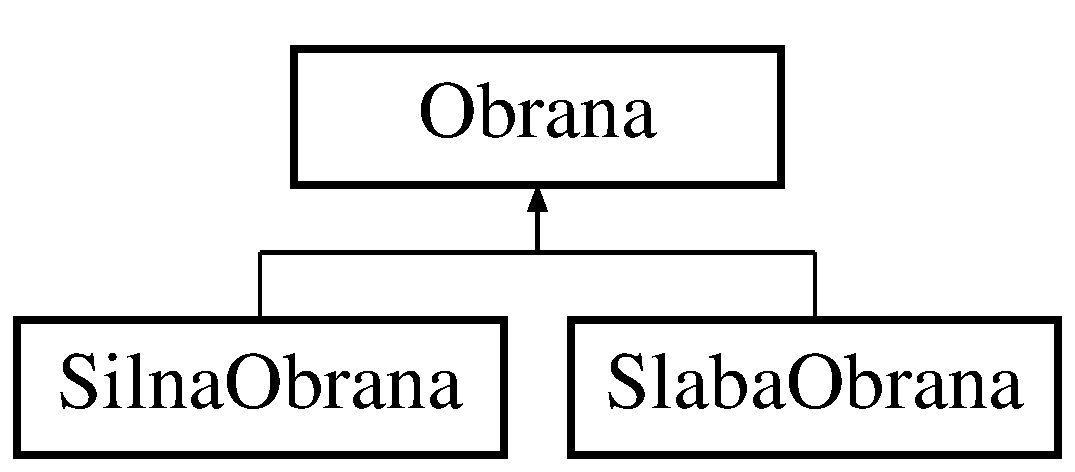
\includegraphics[height=2.000000cm]{class_obrana}
\end{center}
\end{figure}
\subsection*{Public Member Functions}
\begin{DoxyCompactItemize}
\item 
\mbox{\Hypertarget{class_obrana_a8f22b1fbccdd40b2f2b6dfd37b941203}\label{class_obrana_a8f22b1fbccdd40b2f2b6dfd37b941203}} 
{\bfseries Obrana} (int zivot)
\item 
\mbox{\Hypertarget{class_obrana_a0850383cf46b2bbb753fa698482cc893}\label{class_obrana_a0850383cf46b2bbb753fa698482cc893}} 
virtual int {\bfseries get\+Zivot} ()=0
\item 
\mbox{\Hypertarget{class_obrana_ac7c0af7664119702a6228c2375ada964}\label{class_obrana_ac7c0af7664119702a6228c2375ada964}} 
virtual void {\bfseries pridej\+Zivot} ()=0
\item 
\mbox{\Hypertarget{class_obrana_a605003c1b1ce9a792ddbd781284542f4}\label{class_obrana_a605003c1b1ce9a792ddbd781284542f4}} 
virtual void {\bfseries odeber\+Zivot} (int kolik)=0
\item 
\mbox{\Hypertarget{class_obrana_aa951ee2fc287e633ec47e3df50d60f43}\label{class_obrana_aa951ee2fc287e633ec47e3df50d60f43}} 
virtual void {\bfseries print\+Info} ()=0
\end{DoxyCompactItemize}
\subsection*{Protected Attributes}
\begin{DoxyCompactItemize}
\item 
\mbox{\Hypertarget{class_obrana_ab448db043456875d9879338223a4e54a}\label{class_obrana_ab448db043456875d9879338223a4e54a}} 
int {\bfseries m\+\_\+zivot}
\end{DoxyCompactItemize}


The documentation for this class was generated from the following files\+:\begin{DoxyCompactItemize}
\item 
C\+:/\+Users/\+Aleksandre/\+Desktop/\+R\+E\+P\+O\+R\+Z\+I\+T\+A\+R/game\+Code/game\+Lod/Obrana.\+h\item 
C\+:/\+Users/\+Aleksandre/\+Desktop/\+R\+E\+P\+O\+R\+Z\+I\+T\+A\+R/game\+Code/game\+Lod/Obrana.\+cpp\end{DoxyCompactItemize}

\hypertarget{class_pirat}{}\section{Pirat Class Reference}
\label{class_pirat}\index{Pirat@{Pirat}}
\subsection*{Public Member Functions}
\begin{DoxyCompactItemize}
\item 
\mbox{\Hypertarget{class_pirat_a984abc4687cacd66dcb3843a600ff102}\label{class_pirat_a984abc4687cacd66dcb3843a600ff102}} 
{\bfseries Pirat} (\hyperlink{class_zbran}{Zbran} $\ast$zbran, \hyperlink{class_obrana}{Obrana} $\ast$obrana, int bonus)
\item 
\mbox{\Hypertarget{class_pirat_a0e6ded24b8adfb2df2fb13e01b63e5cf}\label{class_pirat_a0e6ded24b8adfb2df2fb13e01b63e5cf}} 
\hyperlink{class_zbran}{Zbran} $\ast$ {\bfseries get\+Zbran} ()
\item 
\mbox{\Hypertarget{class_pirat_ab7f68dad16acecfb6594ffd9447c9e0f}\label{class_pirat_ab7f68dad16acecfb6594ffd9447c9e0f}} 
\hyperlink{class_obrana}{Obrana} $\ast$ {\bfseries get\+Obrana} ()
\item 
\mbox{\Hypertarget{class_pirat_a357e22f0319dfe378b3610ada463dfb5}\label{class_pirat_a357e22f0319dfe378b3610ada463dfb5}} 
int {\bfseries get\+Bonus} ()
\item 
\mbox{\Hypertarget{class_pirat_a0808ef7fc04b9d860afb05f9d77e514f}\label{class_pirat_a0808ef7fc04b9d860afb05f9d77e514f}} 
void {\bfseries print\+Info} ()
\end{DoxyCompactItemize}
\subsection*{Private Attributes}
\begin{DoxyCompactItemize}
\item 
\mbox{\Hypertarget{class_pirat_aee88b4cec2a7ede4e60d2687d70630bb}\label{class_pirat_aee88b4cec2a7ede4e60d2687d70630bb}} 
\hyperlink{class_zbran}{Zbran} $\ast$ {\bfseries m\+\_\+zbran}
\item 
\mbox{\Hypertarget{class_pirat_ad45cfa99580c4ee8a24092b94e73ac8e}\label{class_pirat_ad45cfa99580c4ee8a24092b94e73ac8e}} 
\hyperlink{class_obrana}{Obrana} $\ast$ {\bfseries m\+\_\+obrana}
\item 
\mbox{\Hypertarget{class_pirat_aea6a34a2775e8928c3a968443bfee540}\label{class_pirat_aea6a34a2775e8928c3a968443bfee540}} 
int {\bfseries m\+\_\+bonus}
\end{DoxyCompactItemize}


The documentation for this class was generated from the following files\+:\begin{DoxyCompactItemize}
\item 
C\+:/\+Users/\+Aleksandre/\+Desktop/\+R\+E\+P\+O\+R\+Z\+I\+T\+A\+R/game\+Code/game\+Lod/Pirat.\+h\item 
C\+:/\+Users/\+Aleksandre/\+Desktop/\+R\+E\+P\+O\+R\+Z\+I\+T\+A\+R/game\+Code/game\+Lod/Pirat.\+cpp\end{DoxyCompactItemize}

\hypertarget{class_planeta}{}\section{Planeta Class Reference}
\label{class_planeta}\index{Planeta@{Planeta}}
\subsection*{Public Member Functions}
\begin{DoxyCompactItemize}
\item 
\mbox{\Hypertarget{class_planeta_a986261fdd4028ffb72f19e3adb03d244}\label{class_planeta_a986261fdd4028ffb72f19e3adb03d244}} 
{\bfseries Planeta} (string nazev, int cena\+Za\+Prodej, int cena\+Za\+Nakup, \hyperlink{class_pirat}{Pirat} $\ast$pirat)
\item 
\mbox{\Hypertarget{class_planeta_a1b8778d99a9e6e102b7af3b9411494d7}\label{class_planeta_a1b8778d99a9e6e102b7af3b9411494d7}} 
string {\bfseries get\+Nazev} ()
\item 
\mbox{\Hypertarget{class_planeta_ad6e87052013c2013f765e7914850743a}\label{class_planeta_ad6e87052013c2013f765e7914850743a}} 
\hyperlink{class_suroviny}{Suroviny} $\ast$ {\bfseries get\+Surovina} (int kolikata)
\item 
\mbox{\Hypertarget{class_planeta_a322fc8b1673aa32921db8794ded212b9}\label{class_planeta_a322fc8b1673aa32921db8794ded212b9}} 
\hyperlink{class_lod}{Lod} $\ast$ {\bfseries get\+Lod} ()
\item 
\mbox{\Hypertarget{class_planeta_af53f32a0b7af3d8f6a1094d57e469bda}\label{class_planeta_af53f32a0b7af3d8f6a1094d57e469bda}} 
\hyperlink{class_pirat}{Pirat} $\ast$ {\bfseries get\+Pirat} ()
\item 
\mbox{\Hypertarget{class_planeta_af3757b4e848ce39dbb842d7a750ae5b1}\label{class_planeta_af3757b4e848ce39dbb842d7a750ae5b1}} 
int {\bfseries get\+Cena\+Za\+Prodej} ()
\item 
\mbox{\Hypertarget{class_planeta_abf036d0bf62d574d7d4def69a3668652}\label{class_planeta_abf036d0bf62d574d7d4def69a3668652}} 
int {\bfseries get\+Cena\+Za\+Nakup} ()
\item 
\mbox{\Hypertarget{class_planeta_a3479d0ede2fdaf3d8912de2b95b22d14}\label{class_planeta_a3479d0ede2fdaf3d8912de2b95b22d14}} 
void {\bfseries set\+Lod} (\hyperlink{class_lod}{Lod} $\ast$lod)
\item 
\mbox{\Hypertarget{class_planeta_a3923b1840a785226d82e1057bd9ab6f3}\label{class_planeta_a3923b1840a785226d82e1057bd9ab6f3}} 
void {\bfseries pridej\+Surovinu} (\hyperlink{class_suroviny}{Suroviny} $\ast$surovina)
\item 
\mbox{\Hypertarget{class_planeta_a394655c56d2ba72fdab3720f23e2f31f}\label{class_planeta_a394655c56d2ba72fdab3720f23e2f31f}} 
void {\bfseries odeber\+Surovinu} (int kolikata)
\item 
\mbox{\Hypertarget{class_planeta_a32fb35d5ecc6e98538fd616c7f9dc033}\label{class_planeta_a32fb35d5ecc6e98538fd616c7f9dc033}} 
void {\bfseries boj} (\hyperlink{class_lod}{Lod} $\ast$lod)
\item 
\mbox{\Hypertarget{class_planeta_aded4c9c54fa3266417d3852e435b6464}\label{class_planeta_aded4c9c54fa3266417d3852e435b6464}} 
void {\bfseries nakup\+Surovin} ()
\item 
\mbox{\Hypertarget{class_planeta_ad4b9d4c317d4d984f4bd416a3aea22b6}\label{class_planeta_ad4b9d4c317d4d984f4bd416a3aea22b6}} 
void {\bfseries prodej\+Surovin} ()
\item 
\mbox{\Hypertarget{class_planeta_a05fd163f88a54307ed6ef5345b24f85a}\label{class_planeta_a05fd163f88a54307ed6ef5345b24f85a}} 
void {\bfseries menu} (\hyperlink{class_lod}{Lod} $\ast$lod)
\item 
\mbox{\Hypertarget{class_planeta_aa05930623310c5dfbb5169df606ecae0}\label{class_planeta_aa05930623310c5dfbb5169df606ecae0}} 
void {\bfseries print\+Info} ()
\end{DoxyCompactItemize}
\subsection*{Private Attributes}
\begin{DoxyCompactItemize}
\item 
\mbox{\Hypertarget{class_planeta_a010a965fab8260a481619bf8a20f5fc5}\label{class_planeta_a010a965fab8260a481619bf8a20f5fc5}} 
string {\bfseries m\+\_\+nazev}
\item 
\mbox{\Hypertarget{class_planeta_a0f1ea1020c9c9c28b2a42a8fce3324c3}\label{class_planeta_a0f1ea1020c9c9c28b2a42a8fce3324c3}} 
vector$<$ \hyperlink{class_suroviny}{Suroviny} $\ast$ $>$ {\bfseries m\+\_\+suroviny}
\item 
\mbox{\Hypertarget{class_planeta_a0165a95c2b317ab6679b4674995e5e62}\label{class_planeta_a0165a95c2b317ab6679b4674995e5e62}} 
\hyperlink{class_lod}{Lod} $\ast$ {\bfseries m\+\_\+lod}
\item 
\mbox{\Hypertarget{class_planeta_a3ba0f98683d50d0a254dccf2f0005d4f}\label{class_planeta_a3ba0f98683d50d0a254dccf2f0005d4f}} 
\hyperlink{class_pirat}{Pirat} $\ast$ {\bfseries m\+\_\+pirat}
\item 
\mbox{\Hypertarget{class_planeta_a1167f2e3f48dc202575623da6862de95}\label{class_planeta_a1167f2e3f48dc202575623da6862de95}} 
int {\bfseries m\+\_\+cena\+Za\+Prodej}
\item 
\mbox{\Hypertarget{class_planeta_a0f305cffd46d4c9a441959942b439af5}\label{class_planeta_a0f305cffd46d4c9a441959942b439af5}} 
int {\bfseries m\+\_\+cena\+Za\+Nakup}
\end{DoxyCompactItemize}


The documentation for this class was generated from the following files\+:\begin{DoxyCompactItemize}
\item 
C\+:/\+Users/\+Aleksandre/\+Desktop/\+R\+E\+P\+O\+R\+Z\+I\+T\+A\+R/game\+Code/game\+Lod/Planeta.\+h\item 
C\+:/\+Users/\+Aleksandre/\+Desktop/\+R\+E\+P\+O\+R\+Z\+I\+T\+A\+R/game\+Code/game\+Lod/Planeta.\+cpp\end{DoxyCompactItemize}

\hypertarget{class_silna_obrana}{}\section{Silna\+Obrana Class Reference}
\label{class_silna_obrana}\index{Silna\+Obrana@{Silna\+Obrana}}
Inheritance diagram for Silna\+Obrana\+:\begin{figure}[H]
\begin{center}
\leavevmode
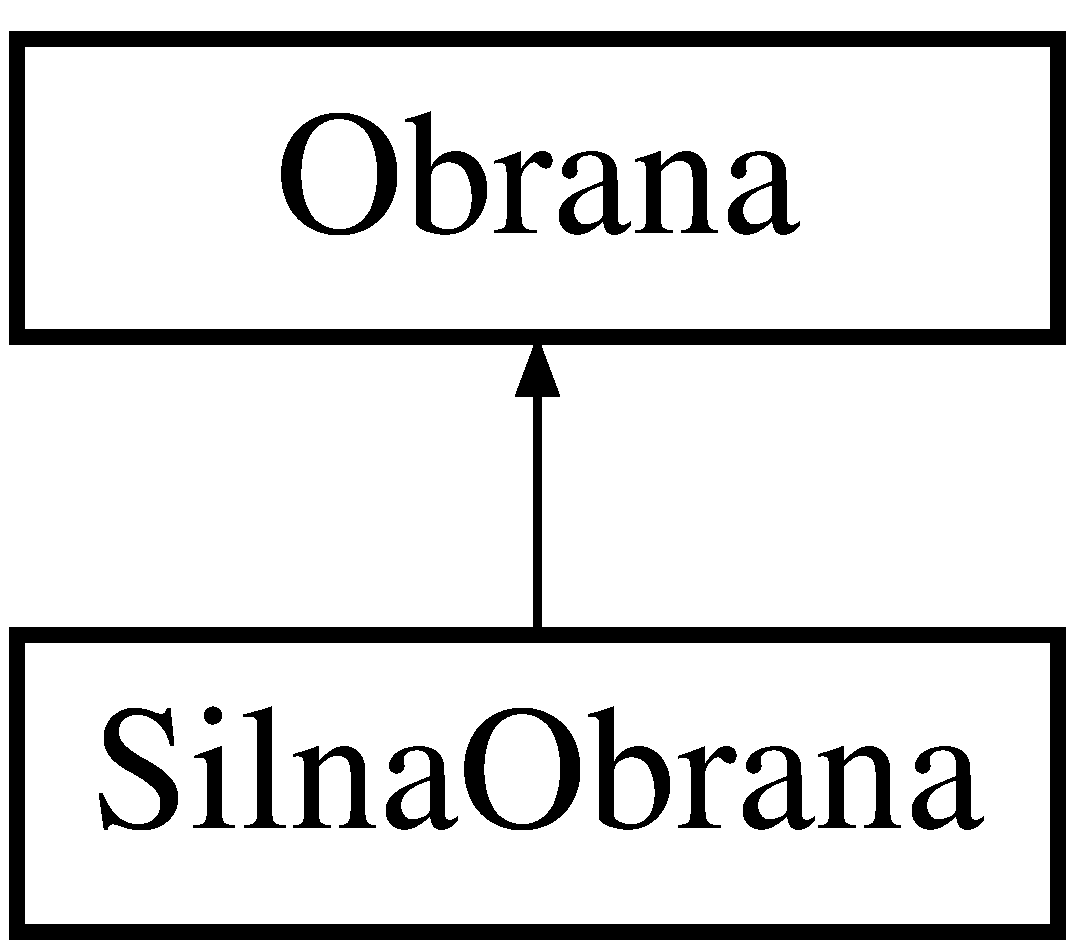
\includegraphics[height=2.000000cm]{class_silna_obrana}
\end{center}
\end{figure}
\subsection*{Public Member Functions}
\begin{DoxyCompactItemize}
\item 
\mbox{\Hypertarget{class_silna_obrana_afeb3f07819fea724a186ac8764133a2a}\label{class_silna_obrana_afeb3f07819fea724a186ac8764133a2a}} 
{\bfseries Silna\+Obrana} (int zivot, int bonus\+Zivota)
\item 
\mbox{\Hypertarget{class_silna_obrana_a156b6f7628df8af5055cf175211dc4e1}\label{class_silna_obrana_a156b6f7628df8af5055cf175211dc4e1}} 
int {\bfseries get\+Zivot} ()
\item 
\mbox{\Hypertarget{class_silna_obrana_a1a7201249cdd63d650f471fa1806a336}\label{class_silna_obrana_a1a7201249cdd63d650f471fa1806a336}} 
void {\bfseries pridej\+Zivot} ()
\item 
\mbox{\Hypertarget{class_silna_obrana_af9c1e2bf4e5035d716eabae03036dfb3}\label{class_silna_obrana_af9c1e2bf4e5035d716eabae03036dfb3}} 
void {\bfseries odeber\+Zivot} (int kolik)
\item 
\mbox{\Hypertarget{class_silna_obrana_af5dcf84053649d61af9b6e364948330b}\label{class_silna_obrana_af5dcf84053649d61af9b6e364948330b}} 
void {\bfseries print\+Info} ()
\end{DoxyCompactItemize}
\subsection*{Public Attributes}
\begin{DoxyCompactItemize}
\item 
\mbox{\Hypertarget{class_silna_obrana_a71f41e0e15e7e77b12eb27657b12abf6}\label{class_silna_obrana_a71f41e0e15e7e77b12eb27657b12abf6}} 
int {\bfseries m\+\_\+bonus\+Zivota}
\end{DoxyCompactItemize}
\subsection*{Additional Inherited Members}


The documentation for this class was generated from the following files\+:\begin{DoxyCompactItemize}
\item 
C\+:/\+Users/\+Aleksandre/\+Desktop/\+R\+E\+P\+O\+R\+Z\+I\+T\+A\+R/game\+Code/game\+Lod/Silna\+Obrana.\+h\item 
C\+:/\+Users/\+Aleksandre/\+Desktop/\+R\+E\+P\+O\+R\+Z\+I\+T\+A\+R/game\+Code/game\+Lod/Silna\+Obrana.\+cpp\end{DoxyCompactItemize}

\hypertarget{class_slaba_obrana}{}\section{Slaba\+Obrana Class Reference}
\label{class_slaba_obrana}\index{Slaba\+Obrana@{Slaba\+Obrana}}
Inheritance diagram for Slaba\+Obrana\+:\begin{figure}[H]
\begin{center}
\leavevmode
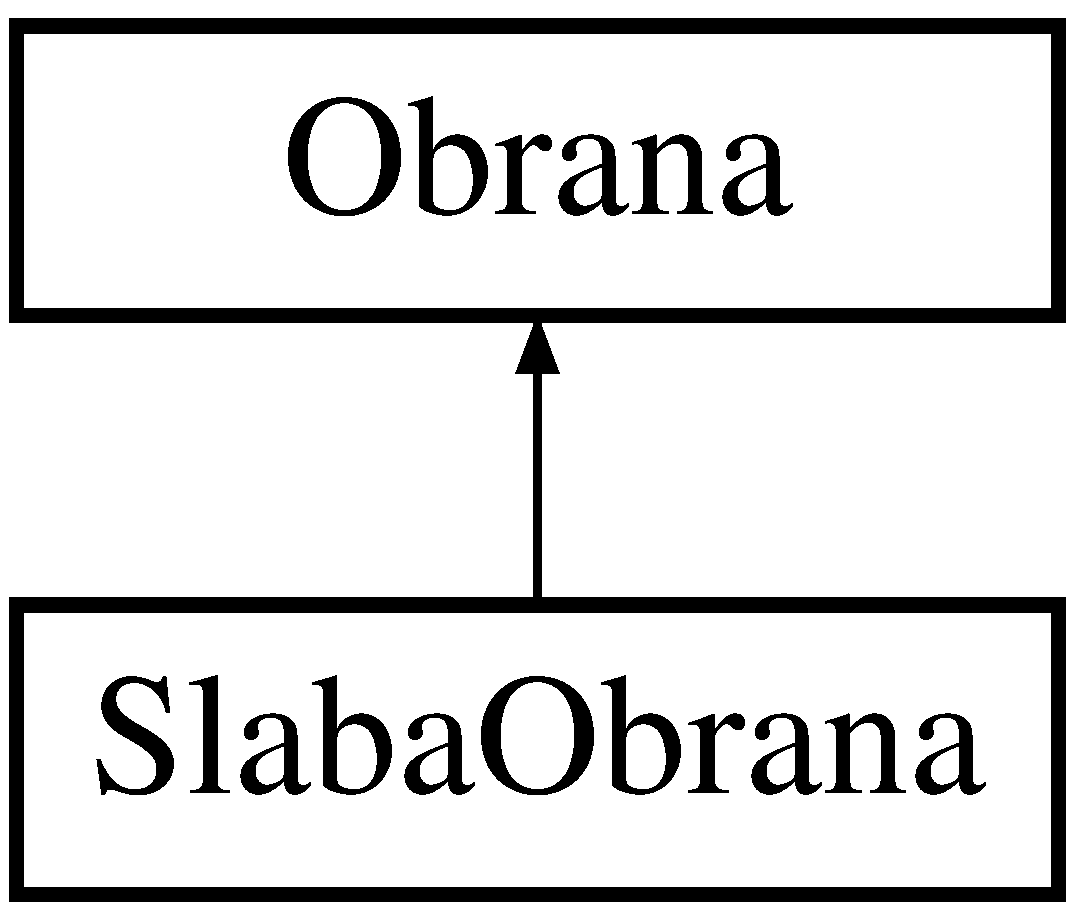
\includegraphics[height=2.000000cm]{class_slaba_obrana}
\end{center}
\end{figure}
\subsection*{Public Member Functions}
\begin{DoxyCompactItemize}
\item 
\mbox{\Hypertarget{class_slaba_obrana_ab2be25cfea788c5be811426b4ec57e7d}\label{class_slaba_obrana_ab2be25cfea788c5be811426b4ec57e7d}} 
{\bfseries Slaba\+Obrana} (int zivot, int bonus\+Zivota)
\item 
\mbox{\Hypertarget{class_slaba_obrana_aa92e97d5c29ce5500f1d981eef43a4b4}\label{class_slaba_obrana_aa92e97d5c29ce5500f1d981eef43a4b4}} 
int {\bfseries get\+Zivot} ()
\item 
\mbox{\Hypertarget{class_slaba_obrana_ade3391029db83c901b6234c75f15b7b0}\label{class_slaba_obrana_ade3391029db83c901b6234c75f15b7b0}} 
void {\bfseries pridej\+Zivot} ()
\item 
\mbox{\Hypertarget{class_slaba_obrana_abc330fc49f131ff5f83a6333e97db94e}\label{class_slaba_obrana_abc330fc49f131ff5f83a6333e97db94e}} 
void {\bfseries odeber\+Zivot} (int kolik)
\item 
\mbox{\Hypertarget{class_slaba_obrana_a3ea5b7c2db7c815676fac8378e188c13}\label{class_slaba_obrana_a3ea5b7c2db7c815676fac8378e188c13}} 
void {\bfseries print\+Info} ()
\end{DoxyCompactItemize}
\subsection*{Public Attributes}
\begin{DoxyCompactItemize}
\item 
\mbox{\Hypertarget{class_slaba_obrana_a95bf94b483018f819856bcd1aab3665c}\label{class_slaba_obrana_a95bf94b483018f819856bcd1aab3665c}} 
int {\bfseries m\+\_\+bonus\+Zivota}
\end{DoxyCompactItemize}
\subsection*{Additional Inherited Members}


The documentation for this class was generated from the following files\+:\begin{DoxyCompactItemize}
\item 
C\+:/\+Users/\+Aleksandre/\+Desktop/\+R\+E\+P\+O\+R\+Z\+I\+T\+A\+R/game\+Code/game\+Lod/Slaba\+Obrana.\+h\item 
C\+:/\+Users/\+Aleksandre/\+Desktop/\+R\+E\+P\+O\+R\+Z\+I\+T\+A\+R/game\+Code/game\+Lod/Slaba\+Obrana.\+cpp\end{DoxyCompactItemize}

\hypertarget{class_suroviny}{}\section{Suroviny Class Reference}
\label{class_suroviny}\index{Suroviny@{Suroviny}}
\subsection*{Public Member Functions}
\begin{DoxyCompactItemize}
\item 
\mbox{\Hypertarget{class_suroviny_a18dcebcaa5e0b5461e60a614d036e5ae}\label{class_suroviny_a18dcebcaa5e0b5461e60a614d036e5ae}} 
{\bfseries Suroviny} (string nazev)
\item 
\mbox{\Hypertarget{class_suroviny_a25629023132f811fb43db7112fe9a436}\label{class_suroviny_a25629023132f811fb43db7112fe9a436}} 
string {\bfseries get\+Nazev} ()
\item 
\mbox{\Hypertarget{class_suroviny_a66975334376d77a96ee1f5d83a35f6d5}\label{class_suroviny_a66975334376d77a96ee1f5d83a35f6d5}} 
void {\bfseries print\+Info} ()
\end{DoxyCompactItemize}
\subsection*{Private Attributes}
\begin{DoxyCompactItemize}
\item 
\mbox{\Hypertarget{class_suroviny_a12dfb3d019df9d1a4a278cad0d2b6bc1}\label{class_suroviny_a12dfb3d019df9d1a4a278cad0d2b6bc1}} 
string {\bfseries m\+\_\+nazev}
\end{DoxyCompactItemize}


The documentation for this class was generated from the following files\+:\begin{DoxyCompactItemize}
\item 
C\+:/\+Users/\+Aleksandre/\+Desktop/\+R\+E\+P\+O\+R\+Z\+I\+T\+A\+R/game\+Code/game\+Lod/Suroviny.\+h\item 
C\+:/\+Users/\+Aleksandre/\+Desktop/\+R\+E\+P\+O\+R\+Z\+I\+T\+A\+R/game\+Code/game\+Lod/Suroviny.\+cpp\end{DoxyCompactItemize}

\hypertarget{class_zbran}{}\section{Zbran Class Reference}
\label{class_zbran}\index{Zbran@{Zbran}}
\subsection*{Public Member Functions}
\begin{DoxyCompactItemize}
\item 
\mbox{\Hypertarget{class_zbran_a06d793187452847683bb0f5bb5542fd1}\label{class_zbran_a06d793187452847683bb0f5bb5542fd1}} 
{\bfseries Zbran} (int sila)
\item 
\mbox{\Hypertarget{class_zbran_acc58bfc8cf0ffa57f3dcd60068bc09dd}\label{class_zbran_acc58bfc8cf0ffa57f3dcd60068bc09dd}} 
int {\bfseries get\+Sila} ()
\item 
\mbox{\Hypertarget{class_zbran_ab226ce4ef3e1a70517c052d3f1953af1}\label{class_zbran_ab226ce4ef3e1a70517c052d3f1953af1}} 
void {\bfseries vylepsit\+Zbran} ()
\item 
\mbox{\Hypertarget{class_zbran_a6185f8a200aed0c3b0396737ca16ce2a}\label{class_zbran_a6185f8a200aed0c3b0396737ca16ce2a}} 
void {\bfseries print\+Info} ()
\end{DoxyCompactItemize}
\subsection*{Private Attributes}
\begin{DoxyCompactItemize}
\item 
\mbox{\Hypertarget{class_zbran_af991ff10f0078033be93c6e2921b5fd3}\label{class_zbran_af991ff10f0078033be93c6e2921b5fd3}} 
int {\bfseries m\+\_\+sila}
\end{DoxyCompactItemize}


The documentation for this class was generated from the following files\+:\begin{DoxyCompactItemize}
\item 
C\+:/\+Users/\+Aleksandre/\+Desktop/\+R\+E\+P\+O\+R\+Z\+I\+T\+A\+R/game\+Code/game\+Lod/Zbran.\+h\item 
C\+:/\+Users/\+Aleksandre/\+Desktop/\+R\+E\+P\+O\+R\+Z\+I\+T\+A\+R/game\+Code/game\+Lod/Zbran.\+cpp\end{DoxyCompactItemize}

%--- End generated contents ---

% Index
\backmatter
\newpage
\phantomsection
\clearemptydoublepage
\addcontentsline{toc}{chapter}{Index}
\printindex

\end{document}
